\chapter{Nigoki: Schedule Replication} \label{chap:schedrep}
In chapter ~\ref{chap:detexec} we described using a deterministic system to ensure the applications on the primary and secondary replica can have the same thread interleaving. The major advantage of the deterministic system is that we can minimize the communication between the replicas. However the downside is that we need to precisely adjust the logical time to maintain decent parallelism for multithreaded applications. We showed various solutions to balance the logical time because we need to keep the execution to be fast and deterministic. If all the burdens come from being deterministic, can we break the determinism once for all but still keep the replicas to be synchronized? The answer is yes.

In this chapter we present Nigoki\footnote{Means Unit 2, in Japanese}: Schedule Replication. In this replication mode, we break the determinism entirely and use messages to synchronize every single synchronization primitives between the primary and replica.

For an application that has massive number of synchronization primitives, this approach might introduce overheads from the communication. Any latency in the the messaging will cause the secondary to fall behind the primary. Fortunately, our system is for inter-kernel replication, and Popcorn Linux provides a messaging layer with relatively low latency (basically memcpy from one kernel to another). As a result having massive massages between replicas won't put too much overhead to the replication.

% !!!!!!!!!put this into conclusion
% \begin{figure}
% \centering
% 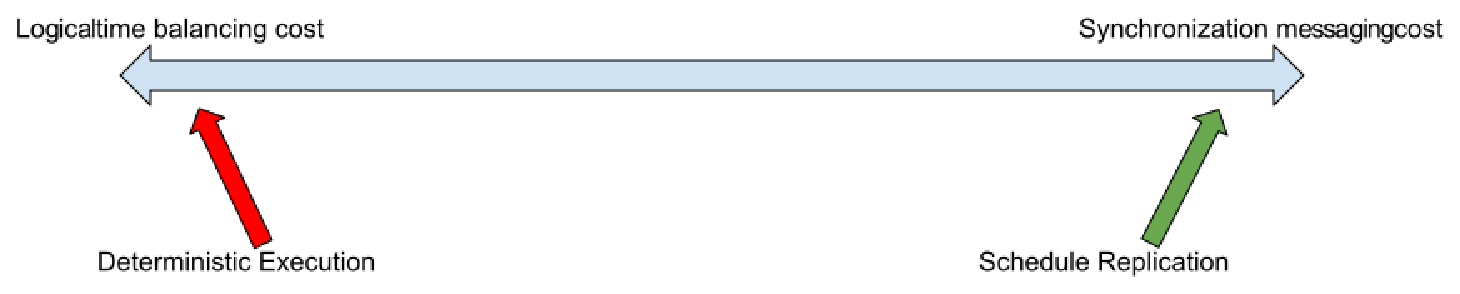
\includegraphics[width=0.8\columnwidth]{figures/tradeoff}
% \caption{Trade off between two algorithms}
% \label{f:tradeoff}
% \end{figure}

\section{Execute-Log-Replay}
Before we get into the detail of this algorithm, let us revisit some important properties that are provided by the deterministic system.

\begin{itemize}
\item Serialization of deterministic sections (the code region between det\_start and det\_end). 
\item Same total order of getting into deterministic sections on primary and secondary.
\end{itemize}

The first property is guaranteed by the fact that the logical time will not change during the execution of a deterministic section, and the second property is guaranteed by increasing the logical time in a same way on both primary and replica. As long as these two properties are guaranteed, the thread interleaving on both primary and secondary are sure to be the same (also for tick bump). By following this paradigm, in our Schedule Replication mode, we guarantee these two properties with the following approaches:

\begin{itemize}
\item Serialize the execution of deterministic sections with a global mutex on both primary and secondary.
\item Log the sequence of getting into deterministic sections on the primary and replay it on the secondary.
\end{itemize}

\begin{figure}
\begin{lstlisting}[numbers=left, frame=single, basicstyle=\small, breaklines]{schedrep}
/*
 * Definitions:
 * ns: current popcorn namespace
 * ns->global_mutex: global_mutex in current namespace
 * ns->seq: global sequence number Seq_global
 * current->seq: task sequence number Seq_thread
 * current->ft_pid: replicated task unique identifier
 */
void __det_start()
{
    if (is_secondary(current))
        wait_for_sync(current->seq, 
            ns->seq, current->ft_pid);
    lock(ns->global_mutex);
    current->ft_det_state = FT_DET_ACTIVE;
}
void __det_end()
{
    if (is_primary(current))
        send_sync(current->seq, 
            ns->seq, current->ft_pid);
    current->seq++;
    ns->seq++;
    current->ft_det_state = FT_DET_INACTIVE;
    unlock(ns->global_mutex);
}
\end{lstlisting}
\caption{Simplified implementation of system calls for schedule replication}
\label{f:schedrep_c}
\end{figure}

% explain something for tha variables
% reference to ft_pid
% why I dont need to handle I/O

Here we still use \detstart\ and \detend\ to wrap around a code section that needs to be synchronized with the replica. Figure~\ref{f:schedrep_c} shows a simplified version of \detstart\ and \detend\ in Schedule Replication.  Every thread in the namespace maintains a sequence number $Seq_{thread}$ and the entire namespace maintains a sequence number $Seq_{global}$. On the primary, \detstart\ simply locks the global mutex, \detend\ unlocks the global mutex, sends a tuple of $< Seq_{thread}, Seq_{global}, ft\_pid >$ to the secondary and then increases the value of $Seq_{global}$ and $Seq_{thread}$. On the secondary, \detstart\ blocks until it receives a $< Seq_{thread}, Seq_{global}, ft\_pid >$ tuple corresponding to its caller thread, then holds the global mutex, and \detend\ increases $Seq_{global}$ and $Seq_{thread}$, then releases the global mutex.

Figure~\ref{f:scherep} shows an example of how Schedule Replication works in action. In this example, T1 on the primary reached \detstart\ first and acquired the global mutex, which blocked T2 from getting into its \detstart\. After the primary reached \detend\, the global mutex is released and T2 was able to proceed. On the secondary, both T1' and T2' got blocked on \detstart\ at the beginning, no matter which one reached its \detstart\ first. T1' was able to proceed after T1 on the primary reached \detend\ and sent the notification to the secondary. T2' proceeded in the same way as T1' did. With this, the timing of calling mutex\_lock on the primary and secondary are synchronized on the primary and secondary.

For each namespace on the secondary, we have a queue for logging the incoming schedule replication message from the primary. The Popcorn message handler for schedule replication message simply appends the message into the queue tail and \detstart\ waits on the queue head to become the schedule sequence that it needs. A crucial prerequisite for this mechanism is that the message in the queue shall preserve strict FIFO sequence. Otherwise an out-of-order message in the queue tail will cause a deadlock in the system, because no \detstart\ will find the matching message in the queue tail. Our implementation guarantees the correct order of the messages, i.e, the messages are put in the queue in a monotonic sequence by their global sequence number $Seq_{global}$.

\begin{itemize}
  \item The synchronization message is sent with the global mutex on hold, this guarantees the monotonic sequence from the sender side.
  \item The messaging layer is strictly FIFO, which will not re-order the messages in its buffer, this guarantees the monotonic sequence from the receiver side.
\end{itemize}

\begin{figure}
\centering
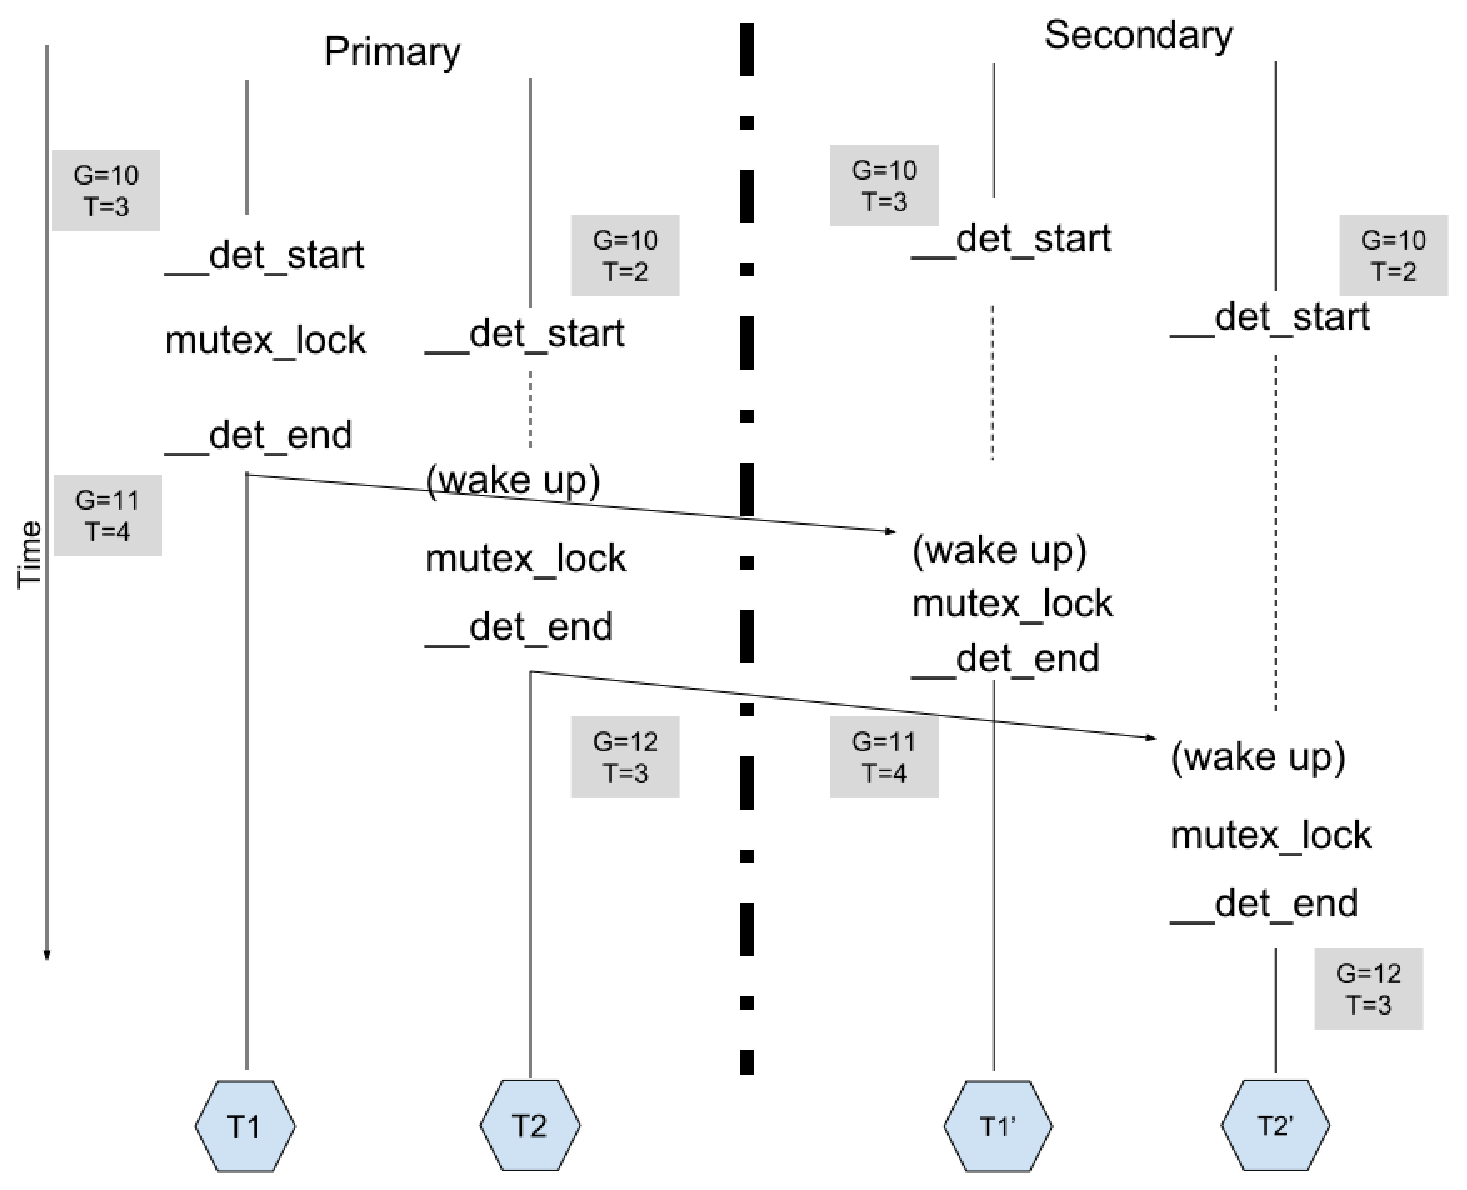
\includegraphics[width=0.9\columnwidth]{figures/sched_rep}
\caption{An example of Schedule Replication}
\label{f:scherep}
\end{figure}

\subsection{Eliminating Deadlocks} \label{sec:rdeadlock}
As we mentioned in Section~\ref{sec:edeadlock}, wrapping all the lock acquisitions with \detstart\ and \detend\ will cause the same deadlock issue, the reason is similar to the case in the Deterministic Execution because we don't release the lock acquisition order when the mutex is contended. The solution in Schedule Replication is similar to what we did in the Deterministic Execution, upon getting into sleep in futex, we release the global mutex and re-acquire it when it wakes up from futex. The futex modification mentioned in Section~\ref{sec:edeadlock} is also applied in this case to ensure the determinism of waking up from futex.

\section{Related Work}
Several previous works also presented the idea of not using a deterministic system for replication. Midas~\cite{slember2006static} points out the non-determinism from both the thread-interleaving and system call outputs, and utilizes a compiler framework to trap those non-deterministic points. The primary records the output of trapped points and replay them on the replica. Rex~\cite{guo2014rex} presents the same idea of logging the lock sequences on the primary and replay it on the replicas. It utilizes Paxos~\cite{lamport2001paxos} to provide a consistent sequence of requests and locks across all the replicas. Comparing to our solution, the advantage of Rex is that it is able to use partial order lock synchronization to provide decent parallelism for different lock acquisitions. But the downside is that both of the solutions are not transparent enough. In Rex, applications need to be manually modified to adopt Rex. (300-500 lines of changes for each application, according to the evaluation part of the paper.) Moreover, both solutions cannot deal with non-determinism from an external library.

A more aggressive idea is not synchronizing the execution sequence at all. EVE~\cite{kapritsos2012all} and Recspec~\cite{lee2010respec} present the idea of running the replica speculatively without synchronizing the thread-interleaving. All of them assume for most of the time the replicas are able to produces the consistent output, but whenever the replica diverges, the diverged one is forced to roll-back to a previous consistent state. Comparing to our solution, EVE is implemented in JAVA and needs a good amount of manual annotation work to the applications. For Recspec, it runs the application and the replicated one inside the same OS, which does not meet the requirement of our use case.

From the fault-tolerance point of view, as replication systems, since EVE~\cite{kapritsos2012all} and Varan~\cite{hosek2015varan} allow the applications to run in different thread-interleavings, an interesting functionality that they can provide is that they are able to tolerate bugs caused by certain thread-interleaving. On those systems, this kind of concurrent bugs can be recovered with the correct run in another thread-interleaving. While in our both replication modes, thread-interleavings are strictly synchronized, the buggy thread-interleaving will also be replicated, which in turns leading to all the replicas to fail. Our scope is limited to tolerating hardware transient fault and assume the applications are bug-free, however, this is still an interesting topic of fault-tolerance to be explored.